\newpage
\section{Continuous Interior Penalty Method}%
\label{sec:continious_interior_penalty_method}






\subsection{Introduction}%
\label{sub:introduction}


To solve \eqref{eq:bi_problem} numerically do we want to introduce the Continuous Interior Penalty Method (CP), which is a Discontinuous Galerkin
method (DG) using $C^{0}$ finite elements. There is several reasons why we want to apply $C^{0}$ instead of the often used
$C^{1}$ finite elements for fourth order problems. First and foremost is the $C^0$ finite elements simpler than
obtaining $C^{1}$ finite elements.  Also, compared to other methods similar to the mixed
finite element method for the problem \eqref{eq:bi_problem}, CP has in fact
preserved the symmetric positive definiteness, which means the stability analysis is more straight forward. Finally and most
importantly according to \cite{brenner2012quadratic} can naive use mixed methods of splitting the boundary conditions of
the problem \eqref{eq:bi_problem} produce wrong solutions if $\Omega $ is non convex.

\todo[inline]{ Write about this: }
\todo[inline]{ Conformal methods $V_{h} \subset V$ requires $C^{1}$. Exists in a good manner in 2D, but does not exist generalization in 3D. Need reference.}
\todo[inline]{Use Bspline as alternative basis. . Less flexible when generating meshes for complicated domains. Need reference.  }
\todo[inline]{ Write in mixed formulation $\overline{w}  = \Delta w$ }
\todo[inline]{ None-conform discretization of 4th order problem using C0 Elements. Hence CP Method }




\subsection{Computational Domains}%
\label{sub:computational_domain}

Let $\mathcal{T}  = \left\{ T \right\} $ be a triangulation of $\Omega \subset   \mathbb{R} ^2 $ consisting of triangles $T$ as in figure \ref{fig:mesh_example}. We may also define the set of all facets $\mathcal{F}_{h}$, where every facet is denoted by $F \in \mathcal{F} _{h}$. However, we will distinguish between the
set of external facets $\mathcal{F}^{ext} _{h}$, which is all facets along $\partial \Omega $, and the interior facets $\mathcal{F} ^{int}_{h}$. Let the facets be denotes as $F \in \mathcal{F } _{h}$, then the normal vector $n$ is across the facets from
$T^{+}$ to $T^{-}$, illustrated in figure \ref{fig:normal}.

\begin{figure}[!h]
\centering
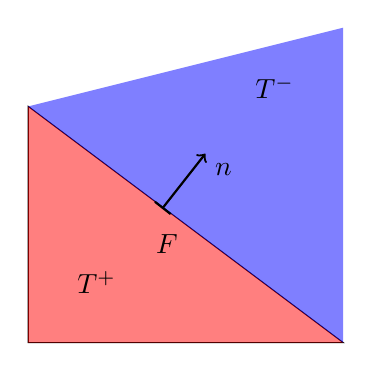
\begin{tikzpicture}[scale=1]
\coordinate (A) at (0,0);
\coordinate (C) at (0,3);
\coordinate (B) at (4,0);
\coordinate (D) at (4,4);
\coordinate (Tm) at (3.5,3.5);
\coordinate (Tp) at (0.5, 0.5);
\coordinate (e) at (1.5, 1.5);
\coordinate (start) at (1.7, 1.7);
\coordinate (end) at (2.25, 2.4);

\draw (A) -- (B) -- (C) -- cycle;
\fill[red, opacity=0.5] (A) -- (B) -- (C);
\fill[blue, opacity=0.5] (B) -- (C) -- (D);
\node[below left] at (Tm) {$T^{-} $ };
\node[above right] at (Tp) {$T^{+}$ };
\node[below right] at (e) {$F$ };

\draw [|->, thick] (start) -- (end);
% \node[above right] at (A) {A };
% \node[below right] at (B) {B};
% \node[above right] at (C) {C };
% \node[below right] at (D) {D};
\node[below right] at (end) {$n$};
\end{tikzpicture}
\caption{Facet $F \in \mathcal{F}_h $ shared by the triangles $T^{+}, T^{-} \in \mathcal{T}_{h} $ and the normal unit vector $n$.  }
    \label{fig:normal}
\end{figure}

A parameter which is useful is the maximum diameter $h$ of the set of triangles $\left\{ T \right\} $, which we to be defined s.t.

\begin{equation}
\begin{split}
    h _{T} & = diam\left( T \right)   = \max_{x_1, x_{2} \in T} dist(x_{1}, x_{2}),  \\
    h_{min} & = \min_{T \in \mathcal{T} } h_{T}, \\
    h_{max} &= \max_{T \in \mathcal{T} }  h_{T} := h,
\end{split}
.\end{equation}

\begin{figure}[!h]
    \centering
    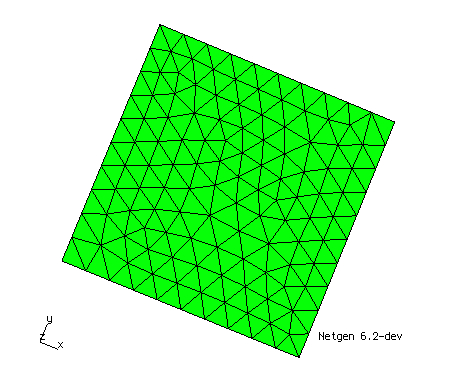
\includegraphics[width=0.45\textwidth]{figures/mesh.jpg}
    \caption{Example of a mesh of $\Omega \subset \mathbb{R} ^{2}$ with triangulation $\mathcal{T} _{h}$.    }
    \label{fig:mesh_example}
\end{figure}

where the $diam( T )$ is the largest facet for a triangle $T$. We will also assume mesh conform i.e., if $T_{1} \neq T_{2 }$  and $T \cap T_{2} \neq \emptyset  $ , then they share either a vertex or a facet.

Let the chunkiness parameter $c_{T} := h_{T}/r_{T}$, where $r_{T}$  is the largest ball that be inscribed inside the element $T$. We can then assume that the mesh is shape-regular i,e., that $c_{T}\le  c$ independent of $T$  and $h$. We may also assuming that
the mesh is quasi-uniform only if it holds that the mesh is shape regular and $h_{max} \le  c h_{min}$.

\todo[inline]{ Why is quasi-uniform important and how does shape regularity affect the numerical solution? }


% \subsection{ Weak Form of Biharmonic Operator in $H^{4} \left( T  \right)$}%
% \label{sub:weak_form_biharmonic_identity_for_triangles}


% Let $w,v \in  H^{4} \left( T  \right) $ and $\mathcal{T}_{h} $ the simplicial triangulation of $\Omega$. Using the same method as in \cite{gu2012c0, brenner2012quadratic} can we
% deduce that for every triangle $T \in  \mathcal{T}_{h} $ it holds that
% \begin{align}
%         \left( \Delta  ^{2} w, v \right) _{T} &= \left< \partial _{n} \nabla ^2 w, v \right>_{\partial T} - \left( \nabla \left( \nabla ^2 w
%  \right), \nabla  v  \right)_{T} \nonumber   \\
% \label{eq:weak_form_identity_1}
%  &= \left( D^2w, D^2v \right)_{T} + \left< \partial _{n} \nabla ^2 w, v \right>_{\partial T}  - \left<\partial _{n}
%  \nabla w, \nabla v \right>_{\partial T} \\
% \label{eq:weak_form_identity_2}
%  &=  \left( D^2 w, D^2 v \right)_{T} - \left<\partial _{nt} w, \partial _{t} v \right>_{\partial T} - \left<\partial
%  _{nn} w, \partial _{n} v \right> _{\partial T} +  \left<\partial _{n} \nabla ^2 w, v \right>_{\partial T}
% .\end{align}
% Note that we in the second step we used that
% \[
%     \begin{split}
% \left( \nabla \left( \nabla ^2 w \right), \nabla  v  \right)_{T} & = \sum_{i=1}^{2}  \int_{T}^{} \left( \nabla \nabla w_{x_{i}} \right)\cdot  v_{x_{i}} \ dx    \\
%  & =  \int_{T}^{} D^2w: D^2v \ dx - \int_{\partial T}^{} \left( \partial _{n} \nabla w \right)
% \cdot  \nabla v  \ ds \\
% &= \left( D^2 w : D^2v  \right) _{ T} + \left<\partial _{n} \nabla w, \nabla v \right>_{\partial T }  \\
%     \end{split}
% \]
% We denote $D^2$ as the Hessian matrix operator such that
% $$( D^2u, D^2v )_{\Omega } = \int_{\Omega }^{} D^{2}u : D^2v  dx,$$
% where $D^2u:D^2v$ is the inner product. Also keep in mind that the last result naturally arise when defining $\nabla  = \left( \partial _{n}, \partial _{t} \right) $ such that
% \[
% \left<\partial _{n} \nabla w, \nabla v \right>_{\partial T} = \left<\partial _{nt} w, \partial _{t} v\right> _{\partial
% T} + \left< \partial _{nn} w, \partial _{n} v  \right> _{\partial T} .
% \]

% Remark that we have two formulations \eqref{eq:weak_form_identity_1} and \eqref{eq:weak_form_identity_2}.


\subsection{Constructing Continuous Interior Penalty Method}%
\label{sub:constructing_continious_interior_penalty_method}

 Let us assume that $u,v \in
H^{4}\left( T  \right) $. Using that the results in \eqref{eq:weak_formulation} also holds for a triangle $T$ can we write
\begin{equation}
\label{eq:bi_basic_dg}
\left( \Delta  ^{2} u,v \right) _{T} =  \left( D^2u,D^2v \right) _{T } - \left(\partial _{nt} u, \partial _{t}v
\right)_{\partial T} - \left(\partial _{nn} u, \partial _{n}v \right)_{\partial T} + \left(\partial _{n} \Delta  u,v
\right)_{\partial T}
.\end{equation}

For global continuity, let  $v \in V =  \left\{ v \in H^{1}\left( \Omega  \right): v_{T} \in  H^{4}\left( T \right), \ \forall T \in
\mathcal{T}_{h}    \right\}   \cap C^{0} (
\Omega  ) $ and $u \in  H^{4}\left( \Omega  \right) $ such that,

\begin{equation}
\label{eq:bi_basic_dg2}
\left( \Delta  ^{2} u,v \right) _{\Omega } = \sum_{T \in  \mathcal{T} _{h}}^{}  \left( D^2u,D^2v \right) _{T } - \left(\partial _{nt} u, \partial _{t}v
\right)_{\partial T} - \left(\partial _{nn} u, \partial _{n}v \right)_{\partial T} + \left(\partial _{n} \Delta  u,v
\right)_{\partial T}.
\end{equation}

However, this can be distinguished to separate integrating over triangles $\mathcal{T} _{h}$ , integrating over exterior facets $\mathcal{F} _{h}^{ext}$ and then integrate interior facets $\mathcal{F} _{h}^{int}$.

\begin{equation}
\label{eq:bi_basic_dg_full_1}
\begin{split}
\left( \Delta  ^{2} u, v \right) _{\Omega } =& \sum_{T \in  \mathcal{T} _{h}}^{} \left( D^2u, D^2v \right)_{T}  + \sum_{F \in \mathcal{F}_{h}^{ext}}  \left(\partial _{n} \Delta u, v  \right) _{F}
- \left(\partial _{nt} u, \partial _{t} v \right) _{F}+
\left( \partial _{nn} u, \partial _{n} v \right)_{F} + \sum_{F \in \mathcal{F}_{h}  ^{int}}^{} \left(\partial _{nn} u , \jump{ \partial _{n} v }
\right)_{F} \\
& = \sum_{T \in  \mathcal{T} _{h}}^{} \left( D^2u, D^2v \right)_{T} + \sum_{F \in
\mathcal{F} ^{ext}_{}}^{} \left<g, v  \right> _{F}
+ \left(n g, \nabla _{n}v \right)_{F}  + \sum_{F \in \mathcal{F}  ^{int}}^{} \left( \partial _{nn} u , \jump{ \partial_{n} v } \right)_{F}
\end{split}
\end{equation}
Keep in mind that any jump over a interior facet $F \subset \mathcal{F} _{h}^{int}   $, visualized in figure \ref{fig:normal}, is defined as $\jump{ a } =    a^{+} - a^{-} $
and similarly will the mean be defined as $\mean{ a  } = \frac{1}{2}(   a^{+}
+ a^{-})$.    The equivalence of \eqref{eq:bi_basic_dg2} and \eqref{eq:bi_basic_dg_full_1} comes from the following argumentation.

\begin{equation*}
    \begin{split}
 \left( \Delta  ^{2} u,v \right) _{\Omega } & =\sum_{T\in \mathcal{T} _{h}}^{} \left( D^2u,D^2v \right) _{T } - \left(\partial _{nt} u, \partial _{t}v
\right)_{\partial T} - \left(\partial _{nn} u, \partial _{n}v \right)_{\partial T} + \left(\partial _{n} \Delta  u,v
\right)_{\partial T} \\
&= \sum_{T\in \mathcal{T} _{h}}^{} \left( D^2u,D^2v \right) _{T } \\
&  \quad + \sum_{F \in \mathcal{F}_{h}^{ext} }^{} \underbrace{\left( \partial _{n} \nabla ^2 u, v  \right)_{E}}_{= \left( g_{2},v \right)_{E} }  -  \underbrace{\left(
\partial _{nt} u, \partial _{t} v \right) _{E}}_{= \left(\partial _{t} g_{1} , \partial _{t}v \right) }  - \underbrace{\left( \partial _{nn} u, \partial _{n} v \right)}_{= \left(n g_{2}, \partial  _{n}v \right)_{F}  }    \\
& \quad  + \sum_{F \in \mathcal{F} _{h}^{int}}^{} \underbrace{\left( \left(\partial _{n^{+}} \nabla ^2 u^{+}
        ,v^{+}\right)_{E}
+ \left(\partial _{n^{-}} \nabla ^2 u^{+} ,v^{-}\right)_{F}  \right)}_{(I)} +
\underbrace{\left( \left(\partial _{n^{+}t} u^{+}, \partial_{t} v^{+} \right)_{F} +  \left(\partial _{n^{-}t} u^{-},
        \partial_{t} v^{-}
\right)_{F}  \right) }_{(II)} +
\underbrace{\left( \left(\partial _{n^{+}n^{+}} u^{+}, v^{+} \right) _{F} + \left(\partial _{n^{-}n^{-}} u^{-}, v^{-}
\right) _{F} \right) }_{(III)}
    \end{split}
.\end{equation*}

Where integration over all interior facets $ \forall E \in \mathcal{F}_{h}^{int}$ is computed in this way:
\begin{equation*}
    \begin{split}
        (I) &  =    \left(\partial _{n^{+}} \nabla ^2 u^{+} ,v^{+}\right)_{F} +
        \left(\partial _{n^{-}} \nabla ^2 u^{+} ,v^{-}\right)_{F} =   \int_{F}^{}
        \jump{ \partial _{n} \nabla ^2 u \cdot v } =
         \int_{F}^{}
         \mean{ \partial _{n} \nabla ^2 u } \underbrace{\jump{ v }}_{= 0}    + \underbrace{\jump{ \partial _{n} \nabla ^2 u
         }}_{= 0}    \mean{ v } = 0 \\
        (II) &  =     \left(\partial _{n^{+}t} u^{+}, \partial_{t} v^{+}
        \right)_{F} +  \left(\partial _{n^{-}t} u^{-}, \partial_{t} v^{-}
\right)_{F}    =   \int_{E}^{}
        \jump{ \partial _{nt} u \cdot  \partial_{t} v } =
         \int_{F}^{}
         \mean{ \partial _{nt} u    } \underbrace{\jump{ \partial_{t} v }  }_{= 0}    + \underbrace{\jump{ \partial
                 _{nt}  u
         }}_{= 0}    \mean{ \partial _{t}v }  = 0\\
        (III) &  =     \left(\partial _{n^{+}n^{+}} u^{+}, \partial_{n^{+}} v^{+} \right)_{F} +  \left(\partial _{n^{-}n^{-}} u^{-}, \partial_{n^{-}} v^{-} \right)_{F}    =    \int_{F}^{} \jump{ \partial _{nn} u \cdot  \partial_{n} v } = \int_{F}^{}
        \mean{ \partial _{nn} u    } \underbrace{\jump{ \partial_{n} v }  }_{\neq 0}    + \underbrace{\jump{ \partial
                 _{nn}  u
         }}_{= 0}    \mean{ \partial _{n}v } =
        \left( \partial _{nn} u    , \jump{ \partial_{n} v } \right)_{F}  \\
    \end{split}
.\end{equation*}

Observe that the cancellations in the term $(I)$ appears of the continuity of $v\in V $ and $u\in H^{4}\left( \Omega  \right) $ which makes the jumps zero. For the second term $(II)$ does the terms become zero cancelled because the tangential
derivative at the facet has no jump. However, The third term $(III)$  is fairly interesting since the discontinuity in normal vector for $v \in V$ is a jump, while the second term is still continuous. It can also be raised that $\mean{ \partial _{nn} u } = \partial _{nn} u  $ holds by the continuity of $H^{4}\left( \Omega  \right) $. Anyhow, the definition of jump of should more interesting when we later weaken the continuity of $u$ during discretization.
Hence, \eqref{eq:bi_basic_dg2} and \eqref{eq:bi_basic_dg_full_1} is equivalent.

\subsection{Formulation of Continious Interior Penalty Method}%
\label{sub:formulation_of_continious_interior_penalty_method}


We can finally start defining the fully discrete formulation. Let the basis be a $\mathcal{P}_{2} $ Lagrange finite element space so,
\[
V_{h} = \left\{ v \in C^{0}\left( \Omega  \right): v_{T} = v | _{T} \in P_{2}\left( T \right), \forall T \in
\mathcal{T}_{h}    \right\}
\]
and
\[
V_{h}^{*} = \begin{cases}
    V_{h} & \text{ if } \alpha  > 0 \\
    \left\{ v \in V_{h}: \int_{\Omega }^{} v dx   = 0   \right\} &  \text{ if } \alpha   = 0
\end{cases}
\]
Now, if we choose $u \in V_{h}$ must we take account that the jump is discrete.
 We have now the final CP formulation.
The discretized numerical problem is to solve $w_{h} \in V_{h}^{*}$ such that
\begin{equation}
\label{eq:CP_A_F}
\mathcal{A}\left( w_{h}, v_{h} \right)   = F\left( v_{h} \right), \quad \forall v_{h} \in V_{h}^{*}  .
\end{equation}
where
\begin{equation}
\label{eq:CP_A_h_1}
\begin{split}
\mathcal{A} \left( w_{h}, v_{h} \right)   =&
  \quad  \left( \alpha  w_{h}, v_{h} \right) _{\Omega }\\
&  + \sum_{T \in \mathcal{T} _{h}}^{} \left( D^2 w_{h}, D^2v_{h} \right) _{T} \\
 & +
  \sum_{E \in \mathcal{F}_{h}^{int} }^{}
  \left< \mean{  \partial _{n n} w_{h} }, \jump{ \partial _{n }v_{h}} \right>_{E}  +
 \left< \mean{ \partial _{n n} v_{h} }, \jump{ \partial _{n}w }      \right>_{E}
+ \frac{\gamma}{h}  \left< \jump{ \partial _{n} w_{h}}, \jump{ \partial _{n} v_{h}   }   \right>_{E}
\end{split}
\end{equation}
and
\begin{equation}
\label{eq:CP_F_h}
F\left( v_{h} \right)  = \left( f, v_{h} \right) _{\Omega } +  \sum_ {\mathcal{F} ^{ext}_{}}^{} \left<g_{2 }, v_{h}  \right> _{E}
+ \left<n g_{2}, \partial  _{n}v_{h} \right>_{E} + \left<\partial _{t} g_{1} , \partial _{t}v_{h} \right>_{E}
\end{equation}
Notice that the regulation term termined by respectively a global tuning parameter $\gamma >0 $ and facet length $h = \left\lvert E \right\rvert $. Another key component to the formulation
in \eqref{eq:CP_A_h_1} after introduction of $ w_{h}, v_{h} \in V^{*}_{h}$  is that we expanded $\left< \partial _{nn}w, \jump{ \partial _{n} v }  \right>_{E} \to \left< \mean{ \partial _{nn}w_{h} }  , \jump{ \partial _{n} v_{h} }  \right>_{E} $ since we can longer not guarantee a
continious jump. For symmetric purposes we also added $ \left< \mean{ \partial _{nn} v_{h}}  , \jump{ \partial _{n} w_{h} }  \right>_{E} $.

We may introduce the compact notation of \eqref{eq:CP_A_h_1}.

\begin{equation}
\label{eq:CP_A_h}
\begin{split}
\mathcal{A} \left( w_{h}, v_{h} \right)   =&
  \quad  \left( \alpha  w_{h}, v_{h} \right) _{\Omega }\\
&  +  \left( D^2 w_{h}, D^2v_{h} \right) _{\mathcal{T} _{h}} \\
 & +
  \left( \mean{  \partial _{n n} w_{h} }, \jump{ \partial _{n }v_{h}} \right)_{\mathcal{F}_{h}}  +
 \left( \mean{ \partial _{n n} v_{h} }, \jump{ \partial _{n}w }      \right)_{\mathcal{F}_{h}}
+ \frac{\gamma }{h}  \left( \jump{ \partial _{n} w_{h}}, \jump{ \partial _{n} v_{h}   }   \right)_{\mathcal{F}_{h}}
\end{split}
\end{equation}

\subsection{Error and Stability Analysis of CP}%
\label{sub:error_and_stability_analysis_of_c0ip}

To guarantee convergence and stability we may want to check coercivity and boundedness of the method.

First of all, let us now establish some important inequalites.
\[
\begin{split}
    \textbf{Cauchy-Schwarz inequality: } & \| ab \|_{  }^{  }  \le \| a \|_{  }^{  } \| b \|_{  }^{  }   \\
    \textbf{Inverse inequality: } & \frac{1}{h}\| \partial _{nn}  v_{h} \|_{\mathcal{F}_{h}   }^{2  }  \le C_{j} \| \nabla ^2 v_{h} \|_{ \mathcal{T} _{h} }^{ 2 }   \\
    \textbf{Youngs epsilon inequality: } & 2ab =   2\sqrt{\varepsilon }a\cdot    \frac{b}{\sqrt{\varepsilon } } \le \varepsilon a^2+ b^2 \frac{1}{\varepsilon }
\end{split}
\]

Let the energy norm be on the form
\begin{equation}
\label{eq:A_energy_norm}
    \begin{split}
\| v_{h} \|_{ h }^{2  } & = \| v_{h} \|_{ a_{h} }^{ 2 } =  \|  w_{h} \|_{ \Omega  }^{  }\| v_{h} \|_{ \Omega  }^{  }  +  \| \nabla ^2 v_{h} \|_{ \mathcal{T} _{h}  }^{ 2 }  + \|  h^{-\frac{1}{2}} \jump{ \partial _{n} v_{h}    }\|_{  \mathcal{F} _{h} }^{  } \\
\| v \|_{ h }^{ 2 }  &= \| v \|_{ a_{h},* }^{ 2 } = \| v \|_{ a_{h} }^{ 2 }  + \| h^{\frac{1}{2}} \left\{ \partial _{nn } v\right\}  \|_{ F  }^{  }, \quad  v\in V \oplus V_{h}
    \end{split}
.\end{equation}
The method is said to be coercive if $\mathcal{A} _{h}\left( v_{h}, v_{h} \right) \ge  C \| v_{h} \|_{ a_{h} }^{  } $. Similarly, it is bounded if $ \mathcal{A} _{h} \left( v_{h}, u_{h} \right) \le  C \| u_{h} \|_{  a_{h}}^{ 2 }  \| v_{h} \|_{ a_{h}
}^{ 2 } $ and then, according to Lax Milgram (need reference), the solution does exist and be unique.

\subsubsection{Coercitivity}%
\label{ssub:coercitivity}


Suppose we have the CP problem described in \eqref{eq:CP_A_F}. Then is the coercivity be computed such that
\[
    \begin{split}
\mathcal{A} \left( v_{h}, v_{h} \right) & =\alpha \|  w_{h}  v_{h} \|_{ \Omega  }^{  } +  \| D^2v_{h} \|_{ \mathcal{T} _{h} }^{2  }  + 2 \left(  \mean{ \partial _{nn} v_{h} }    ,  \jump{ \partial _{n}v_{h} }     \right) _{\mathcal{F} _{h}} +  \frac{\gamma}{h} \|  \jump{ \partial _{n} v_{h} }
  \|_{ \mathcal{F} _{h} }^{ 2 } \\
\quad \textit{Cauchy-Schwarz inequality} \quad
& \ge \alpha \| w_{h}  \|_{\Omega   }^{  } \| v_{h} \|_{\Omega   }^{  } +   \| D ^2 v_{h} \|_{ \mathcal{T} _{h} }^{2  } -2 \| h^{\frac{1}{2}} \mean{ \partial _{nn}v_{h} }    \|_{  \mathcal{F} _{h}}^{  } \| h^{-\frac{1}{2}} \jump{ \partial _{n}v_{h} }    \|_{  \mathcal{F} _{h}}^{  } + \gamma \| h^{-\frac{1}{2}}  \jump{ \partial _{n}v_{h} }   \|_{ \mathcal{F} _{h}  }^{ 2 } \\
\quad \textit{Inverse inequality} \quad
 &  \ge \alpha \| w_{h}  \|_{\Omega   }^{  } \| v_{h} \|_{\Omega   }^{  } + \| D ^2 v_{h}  \|_{ \mathcal{T} _{h}  }^{ 2  } - 2 C^{\frac{1}{2}}_{j} \|   D ^2 v_{h}    \|_{ \mathcal{T} _{h}  }^{  } \| h^{-\frac{1}{2}} \jump{ \partial _{n} v_{h} }   \|_{ \mathcal{F} _{h} }^{  }  + \gamma \| h^{ -\frac{1}{2}} \jump{
 \partial _{n } v_{h}}   \|_{ \mathcal{F}_{h}}^{2}  \\
\quad \textit{ Youngs epsilon inequality} \quad
  &  \ge\alpha \| w_{h}  \|_{\Omega   }^{  } \| v_{h} \|_{\Omega   }^{  } +  \| D ^2 v_{h} \|_{ \mathcal{T}_{h}  }^{2  } - \varepsilon C_{j} \| D ^2 v_{h} \|_{ \mathcal{T} _{h} }^{2  } - \frac{1}{\varepsilon } \| h^{\frac{1}{2}} \jump{ \partial _{n} v_{h} }   \|_{ \mathcal{F} _{h} }^{2  }  + \gamma \|
  h^{-\frac{1}{2}} \jump{ \partial _{n} v_{h}}   \|_{ \mathcal{F} _{h} }^{2  }  \\
  & =  \alpha \| w_{h}  \|_{\Omega   }^{  } \| v_{h} \|_{\Omega   }^{  } +\left( 1 - \varepsilon C_{j} \right) \| D ^2 v_{h} \|_{\mathcal{T} _{h}  }^{ 2 } + \left( \gamma  - \frac{1}{\varepsilon } \right) \| h^{-\frac{1}{2}} \jump{ \partial _{n} v_{h} }   \|_{ \mathcal{T} _{h} }^{ 2 } \\
  (\varepsilon  = \frac{1}{2 C_{j} })  \implies  \quad \quad &= \alpha \| w_{h}  \|_{\Omega   }^{  } \| v_{h} \|_{\Omega   }^{  } +\frac{1}{2} \| D ^2 v_{h} \|_{ \mathcal{T} _{h} }^{ 2 }  + \underbrace{\left( \gamma -2 C_{j} \right)}_{ \ge  \frac{1}{2}}  \| h^{\frac{1}{2}} \jump{ \partial _{n} v_{h} }   \|_{
  \mathcal{F} _{h} }^{  } \ge C \| v_{h} \|_{ a_{h} }^{  2}
    \end{split}
\]
This holds if $C=\min\left\{  \alpha , 1 /2\right\}$.
Observe that for the first inequality is the standard \textbf{Cauchy-Schwarz inequality} such that $$\left( \mean{ \partial_{nn} v_{h} }  , \jump{ \partial _{n} v_{h} }   \right) _{\mathcal{F} _{h}} \ge - \| h^{-\frac{1}{2}} \mean{ \partial _{nn}
v_{h} }    \|_{\mathcal{F}_{h}   }^{  } \| \mean{ \partial _{n}v_{h} }   \|_{ \mathcal{F}_{h}   }^{  } .  $$ On the second inequality the \textbf{Inverse inequality} was applied,
\[
- \| h^{\frac{1}{2}} \mean{ \partial _{nn}v }   \|_{ \mathcal{F} _{h}  }^{  }\ge - C_{j}^{\frac{1}{2}} \| D ^2 v_{h} \|_{ \mathcal{T} _{h} }^{  }
\]
The next step is then to use the \textbf{Youngs epsilon inequality} to be able to separate the facets and triangulation norms. \[
 - 2 C^{\frac{1}{2}}_{j} \|  D ^2 v_{h}    \|_{ \mathcal{T} _{h}  }^{  } \| h^{\frac{1}{2}} \jump{ \partial _{n} v_{h} }   \|_{ \mathcal{F} _{h} }^{2  } \ge- \varepsilon C_{j} \| D ^2 v_{h} \|_{ \mathcal{T} _{h} }^{2  } -
 \frac{1}{\varepsilon } \| h^{\frac{1}{2}} \jump{ \partial _{n} v_{h} }   \|_{ \mathcal{F} _{h} }^{2  }
\]
The last step was to choose a $\varepsilon $ and $\gamma $ as some positive constant so that the second term is restricted to be multiplied with something bigger than $\frac{1}{2}$. Thus, the term fulfils coercivity of the \eqref{eq:A_energy_norm}. Hence, the CP method is coercive.

\subsubsection{Boundedness}%
\label{ssub:bounded}
We want the CP method to be bounded.
\begin{equation*}
    \begin{split}
\mathcal{A} \left( w_{h}, v_{h} \right)   =& \left( \alpha w_{h}, v_{h} \right) _{\Omega } +
    \left( D ^2 w_{h}, D ^2v_{h} \right) _{\mathcal{T} _{h}}
  +
  \left( \mean{  \partial _{n n} w_{h} }, \jump{ \partial _{n }v_{h}} \right)_{\mathcal{F}_{h}}  +
 \left( \mean{ \partial _{n n} v_{h} }, \jump{ \partial _{n}w }      \right)_{\mathcal{F}_{h}} \\
 & + \frac{\gamma }{h}  \left( \jump{ \partial _{n} w_{h}}, \jump{ \partial _{n} v_{h}   }   \right)_{\mathcal{F}_{h}} \\
\quad \textit{Cauchy-Schwarz inequality }\quad  &\le \alpha  \|  w_{h} \|_{\Omega   }^{  } \| v_{h} \|_{ \Omega  }^{  }     +
\| D ^2w_{h} \|_{\mathcal{T} _{h}   }^{  }  \| D ^2v_{h} \|_{\mathcal{T} _{h}   }^{  } + \| h^{\frac{1}{2}}\mean{ \partial _{nn} w_{h} } \|_{ \mathcal{F}_{h}  }^{  } \| h^{-\frac{1}{2}}\jump{ \partial _{n} v_{h} } \|_{ \mathcal{F}_{h}  }^{  }    \\
& \quad  + \| h^{\frac{1}{2}}\mean{ \partial _{nn} v_{h} }
\|_{ \mathcal{F}_{h}  }^{  } \| h^{-\frac{1}{2}}\jump{ \partial _{n} w_{h} } \|_{ \mathcal{F}_{h}  }^{  } + \gamma \| h^{-1} \jump{ \partial _{n} v_{h}}   \|_{ \mathcal{F} _{h} }^{  }   \|  \jump{ \partial _{n} w_{h}}   \|_{ \mathcal{F} _{h} }^{  } \\
\quad \textit{Inverse inequality }\quad  &\le \alpha  \|  w_{h} \|_{\Omega   }^{  } \| v_{h} \|_{ \Omega  }^{  }  +
\| D ^2w_{h} \|_{\mathcal{T} _{h}   }^{  }  \| D ^2v_{h} \|_{\mathcal{T} _{h}   }^{  } + C_{j}^{\frac{1}{2}} \| D ^2 w_{h} \|_{\mathcal{T} _{h}  }^{  }  \| h^{-\frac{1}{2}}\jump{ \partial _{n} v_{h} } \|_{ \mathcal{F}_{h}  }^{  }   +
 \\
& \quad  C_{j}^{\frac{1}{2}} \| D ^2 w_{h} \|_{\mathcal{T} _{h}  }^{  }
 \| h^{-\frac{1}{2}}\jump{ \partial _{n} w_{h} } \|_{ \mathcal{F}_{h}  }^{  } + \gamma \| h^{-1} \jump{ \partial _{n} v_{h}}   \|_{ \mathcal{F} _{h} }^{  }   \|  \jump{ \partial _{n} w_{h}}   \|_{ \mathcal{F} _{h} }^{  } \\
\textit{ Using \eqref{eq:bounded_ineq}}  \quad & \le\alpha  \|  w_{h} \|_{a_{h}   }^{  } \| v_{h} \|_{ a_{h}   }^{  } + \| w_{h} \|_{ a_{h} }^{  } \| v_{h} \|_{ a_{h} }^{  }  + 2C_{j}^{\frac{1}{2}} \| w_{h} \|_{ a_{h} }^{  } \| v_{h} \|_{ a_{h} }^{  } + \gamma \| v_{h} \|_{ a_{h} }^{  } \| w_{h} \|_{ a_{h} }^{  } \\
& \le  \left( \alpha + 1 + 2C_{j}^{\frac{1}{2}} + \gamma  \right)  \| v_{h} \|_{a_{h}  }^{  }  \| w_{h} \|_{ a_{h} }^{  }  \le  K  \| v_{h} \|_{a_{h}  }^{  }  \| w_{h} \|_{ a_{h} }^{  }
\end{split}
\end{equation*}

Thus, the CP method is shown to be bounded.
Again, the first step was to apply the \textbf{Cauchy-Schwarz inequality} for every term. On the second inequality the \textbf{Inverse inequality} was applied so that
\[
\| h^{\frac{1}{2}} \mean{ \partial _{nn}v_{h} }   \|_{ \mathcal{F} _{h}  }^{  }\le   C_{j}^{\frac{1}{2}} \| D ^2 v_{h} \|_{ \mathcal{T} _{h} }^{  } \quad \text{and} \quad   \| h^{\frac{1}{2}} \mean{ \partial _{nn}w_{h} }   \|_{ \mathcal{F} _{h}
}^{  }\le   C_{j}^{\frac{1}{2}} \| D ^2 w_{h} \|_{ \mathcal{T} _{h} }^{  }.
\]
The second step can we luckily observe that all terms invidually is less than the norm such that
\begin{equation}
\label{eq:bounded_ineq}
\begin{split}
\| w_{h} \|_{\Omega    }^{  }  \| v_{h} \|_{ \Omega    }^{  } & \le \| w_{h} \|_{ a_{h} }^{  } \| v_{h} \|_{ a_{h} }^{  }, \\
\| D ^2w_{h} \|_{\mathcal{T}_{h}   }^{  }  \| D ^2v_{h} \|_{\mathcal{T}_{h}   }^{  } & \le \| w_{h} \|_{ a_{h} }^{  } \| v_{h} \|_{ a_{h} }^{  }, \\
\|  D ^2 w_{h} \|_{ \mathcal{T} _{h} }^{ } \| h^{-\frac{1}{2}} \jump{ \partial _{n} v_{h} }   \|_{ \mathcal{F} _{h} }^{  }  & \le  \| w_{h} \|_{ a_{h} }^{  } \| v_{h} \|_{ a_{h} }^{  }, \quad  \|  D ^2 v_{h} \|_{ \mathcal{T} _{h} }^{ } \| h^{-\frac{1}{2}} \jump{ \partial _{n} w_{h} }   \|_{ \mathcal{F} _{h} }^{  }   \le \| v_{h} \|_{ a_{h} }^{  } \| w_{h} \|_{ a_{h} }^{  }, \\
\text{and} \quad    \gamma \| h^{-1 } \jump{ \partial _{n} v_{h} }   & \|_{ \mathcal{F} _{h}  }^{  }  \| \jump{ \partial _{n} w_{h} }    \|_{\mathcal{F}_{h}   }^{  }   \le \gamma \| v_{h} \|_{ a_{h} }^{  }  \| w_{h} \|_{ a_{h} }^{  }.
\end{split}
\end{equation}
Hence, the CP method is does fulfills the Lax Milgram criteria because it is both bounded and unique.


\subsection{Apriori Estimates}%
\label{sub:apriori_estimates}

We will now introduce the notion of an apriori estimate, which can be used the estimate the size of a solution even before we have a solution. However, we will first introduce some basic results from the theory of Galerkin methods.

\subsubsection{Galerkin Orthogonality}%
\label{ssub:galerkin_orthonality}

Let us recall the weak continuous problem \eqref{eq:continious_problem} and the weak discrete problem \eqref{eq:discrete_problem}.
\begin{align}
    \label{eq:continious_problem}
    \text{Find } u \in V \quad&  \text{s.t. } a\left( u,v \right) = l\left( v \right)  \quad \forall v \in V. \\
    \label{eq:discrete_problem}
    \text{Find } u_h \in V_h \quad&  \text{s.t. } a\left( u_h,v_h \right) = l\left( v_h \right)  \quad \forall v_h \in V_h.
.\end{align}

In fact, the key property of this problem formulation is that $a\left( u, v_{h} \right)  = l \left( v_{h} \right) \quad  \forall v_{h} \in V_{h} \subset V  $. Thus, the Galerkin orthogonality property holds so that,
$$
a\left( u, v_{h} \right)  - a\left( u_{h}, v_{h} \right) = a\left( u- u_{h}, v_{h} \right) = 0,   . $$
Keep in mind that we define
$ u - u_{h} \in V$
\subsubsection{Céa's Lemma }%
\label{ssub:ceas_lemma}

Assume that the problems \eqref{eq:continious_problem} and \eqref{eq:discrete_problem} satisfied the Lax Milgram criteria,
\begin{equation*}
    \begin{split}
a\left( u,v \right)  & \le C \| u \|_{  }^{  }  \| v \|_{  }^{  }  \quad   \left( V_{h} \right) , \quad  \alpha \|  u\|_{   }^{     2} \le a \left( u,u \right) \quad \forall u,v\in V, \\
a\left( u_{h},v_{h} \right)  & \le C \| u_{h} \|_{  }^{  }  \| v_{h} \|_{  }^{  }   \left( V_{h} \right) , \quad  \alpha \| u_{h}\|_{   }^{     2} \le a \left( u_{h},u_{h} \right)\quad  \forall u_{h},v_{h}\in V_{h}.
    \end{split}
.\end{equation*}

Then the Céa's lemma says that this is satisfied,
\begin{equation}
\label{eq:Ceas_lemma_continious}
\| u - u_{h} \|_{  }^{  } \le \frac{C}{\alpha }  \inf_{v_{h} \in V_{h}} \| v_{h} - v \|_{  }^{  } .
\end{equation}

The lemma naturally arise using the following argumentation,
\begin{equation}
\label{eq:cealemma_proof}
    \begin{split}
\alpha \| u - u_{h} \|_{  }^{  2} & \le a\left( u-u_{h}, u - u_{h} \right) \\
&= a\left( u - u_{h}, u - v_{h} \right)  - a\left( u - u_{h}, v_{h} - u_{h} \right)  \\
& \le  C\| u - u_{h} \|_{  }^{  } \| u - v_{h} \|_{  }^{  } \\
\implies &  \alpha \| u - u_{h} \|_{  }^{  }    \le  C \| v_{h} - u \|_{  }^{  } \le C \inf_{v_{h} \in V_{h}} \| v_{h} -u \|_{  }^{  }.
    \end{split}
.\end{equation}

\subsubsection{Céa's Lemma for CP Method, }%
\label{ssub:ceas_lemma}
Since we have discrete coercivity, then $V_{h} \not \subset V$, thus the standard method does not work. Firstly, we want to use the results from \ref{sub:error_and_stability_analysis_of_c0ip}. We have shown that
\begin{equation*}
    \begin{split}
    \textit{Discrete coercivity } \quad & \hat{\alpha } \| u_{h} \|_{ a_{h} }^{ 2 }  \le  \mathcal{A} \left( u_{h}, u_{h} \right) \\
    \textit{Boundedness (semi-discrete) }\quad  & \mathcal{A} \left( v,w_{h} \right)  \le  \widetilde{C} \| v \|_{ a_{h,*} }^{  }  \| w_{h} \|_{ a_{h} }^{  } \quad \forall v \in  V_{h} \oplus H^{4}\left( \Omega  \right) \\
    \textit{Boundedness (fully discrete) }\quad  & \mathcal{A} \left( v_{h},w_{h} \right)  \le  \overline{C}  \| v \|_{ a_{h,*} }^{  }  \| w_{h} \|_{ a_{h} }^{  } \quad \forall v_{h}, w_{h} \in V_{h}
    \end{split}
.\end{equation*}

Let the difference have the form $u - u_{h} = (u - v_{h} )  + (v_{h} - u_{h})$ and the define identity
$$
\| w_{h} \|_{ a_{h,*} }^{  }  \le  D \| w_{h} \|_{ a_{h} }^{  }, \forall w_{h} \in V_{h} .
$$


Thus, the norm can now be computed such that\[
\| u - u_{h} \|_{ a_{h,*} }^{  } \le \|u - v_{h}  \|_{a_{h,*}  }^{  }  + \| v_{h} - u_{h} \|_{a_{h,*}  }^{  } \\
\le \| u -v_{h} \|_{ a_{h,*} }^{  }  + D \| u_{h} - v_{h} \|_{a_{h}  }^{  }.
\]

Finally, following the same procedure as in \eqref{eq:cealemma_proof} we get
\[
    \begin{split}
\| u_{h} - v_{h} \|_{a_{h}  }^{2  } \hat{\alpha } & \le  \mathcal{A} \left( u_{h} - v_{h}, u_{h} - v_{h} \right) \\
& =  \mathcal{A} _{h} \left( u_{h} -u, u_{h} -v_{h} \right) + \mathcal{A} \left( u - v_{h}, u_{h} - v_{h} \right) \\
 &  \le  \mathcal{A}  \left( u - v_{h}, u_{h} - v_{h} \right)   \\
 &\le  \widetilde{C} \| u - v_{h} \|_{ a_{h,*} }^{  } \| u- v_{h} \|_{ a_{h} }^{  }
    \end{split}
\]
Observe that we now have $ \| u_{h} - v_{h} \|_{ a_{h} }^{  }   \le \frac{\widetilde{C}}{\hat{\alpha }}  \| u - v_{h} \|_{ a_{h, *} }^{  }$ and $\| u - u_{h} \|_{ a_{h,*} }^{  }   \le \left( 1 + D \widetilde{C} /\hat{\alpha } \right)\cdot  \| u - v_{h} \|_{ a_{h,*} }^{  } $. Hence, we have derived a equivalent Céa's lemma for the CP method.
\[
    \begin{split}
\| u_{h} - v_{h} \|_{ a_{h} }^{  }  & \le \frac{\widetilde{C}}{\hat{\alpha }}  \inf_{v_{h} \in  V_{h}} \|  v_{h} - u \|_{ a_{h, *} }^{  } \\
\| u - u_{h} \|_{ a_{h,*} }^{  }  & \le \left( 1 + D \widetilde{C} /\hat{\alpha } \right)\cdot \inf_{v_{h} \in  V_{h}}   \| u - v_{h} \|_{ a_{h,*} }^{  }
    \end{split}
\]


\newpage
\section{Numerical Results}%
\label{sec:numerical_results}

\subsection{Manufactured Solution}%
\label{sub:manufactured_solution}

\subsection{Convergence Rate}%
\label{sub:convergence_rate}

\subsection{Condition Number}%
\label{sub:condition_number}



\section{HCP Method copied from NGSolve}%
\label{ssub:hc0ip_method_from_ngsolve}

We consider the Kirchhoff plate equation: Find $w \in H^2$, such that

$$
\int \nabla^2 w : \nabla^2 v = \int f v
$$

A conforming method requires $C^1$ continuous finite elements. But there is no good option available, and thus there is no $H^2$ conforming finite element space in NGSolve.

$$
\sum_T \nabla^2 w : \nabla^2 v
- \int_{E} \{\nabla^2 w\}_{nn} \, [\partial_n v]
- \int_{E} \{\nabla^2 v\}_{nn} \, [\partial_n w] + \alpha \int_E  [\partial_n w]  [\partial_n v]
$$

[Baker 77, Brenner Gudi Sung, 2010]

We consider its hybrid DG version, where the normal derivative is a new, facet-based variable:


$$
\sum_T \nabla^2 w : \nabla^2 v
- \int_{\partial T} (\nabla^2 w)_{nn} \, (\partial_n v - \widehat{v_n})
- \int_{\partial T} (\nabla^2 v)_{nn} \, (\partial_n w - \widehat{w_n}) + \alpha \int_E (\partial_n v - \widehat{v_n}) (\partial_n w - \widehat{w_n})
$$






